%% Flux — the short introduction.
%% A compression of the 422-page technical paper. Shares its numbers and its macros;
%% every figure here must be greppable in ../paper and match. See plan/short-paper.md.
\documentclass[11pt,a4paper]{article}

\usepackage[utf8]{inputenc}
\usepackage[T1]{fontenc}
\usepackage{lmodern}
%% Wider margins and more leading than the long paper: this one is read linearly,
%% not consulted.
\usepackage[margin=1.15in]{geometry}
\linespread{1.06}
\usepackage{amsmath,amssymb,amsthm}
\usepackage{booktabs}
\usepackage{array}   %% >{\raggedright\arraybackslash} column specifiers
\usepackage{siunitx}
\usepackage{xcolor}
\usepackage{float}
\usepackage{tikz}
\usetikzlibrary{arrows.meta,positioning,fit,backgrounds,calc}
\usepackage{xspace}
\usepackage{microtype}
\usepackage{titlesec}
\usepackage{fancyhdr}
\usepackage{enumitem}
\usepackage[colorlinks=true]{hyperref}
\usepackage[capitalise,nameinlink]{cleveref}

\sisetup{group-separator={,},group-minimum-digits=4,group-digits=integer}
\setlength{\emergencystretch}{3em}

%% Same palette as the long paper, so the two read as siblings.
\definecolor{FluxBlue}{HTML}{1F4E79}
\definecolor{FluxSlate}{HTML}{44546A}
\definecolor{FluxRule}{HTML}{BFC7D2}
\definecolor{FluxSettled}{HTML}{2E7D32}
\definecolor{FluxGap}{HTML}{5F6368}
\definecolor{FluxProposed}{HTML}{1565C0}

\hypersetup{linkcolor=FluxBlue,citecolor=FluxBlue,urlcolor=FluxBlue,
  pdftitle={Flux: A Decentralized Cloud for Autonomous Compute — a short introduction},
  pdfauthor={Tadeas Kmenta}}

\pagestyle{fancy}\fancyhf{}
\renewcommand{\headrulewidth}{0.4pt}
\fancyhead[L]{\footnotesize\color{FluxSlate}\nouppercase{\leftmark}}
\fancyhead[R]{\footnotesize\color{FluxSlate}\thepage}
\renewcommand{\sectionmark}[1]{\markboth{\thesection\quad #1}{}}

\titleformat{\section}[hang]{\Large\bfseries\color{FluxBlue}}{\thesection}{0.7em}{}
\titleformat{\subsection}[hang]{\large\bfseries\color{FluxSlate}}{\thesubsection}{0.6em}{}
\titlespacing*{\section}{0pt}{2.8ex plus 1ex}{1.5ex}

%% Shared macros: component names, symbols, maturity tags. Reused rather than
%% redefined so the two documents cannot drift apart on terminology.
%% ---------------------------------------------------------------------------
%% notation.tex — canonical names, symbols, units and theorem environments.
%% EVERY drafter uses these macros and NO others. Naming conflicts across the
%% Flux repositories are decided here, once, and nowhere else.
%% ---------------------------------------------------------------------------

%% ======================= theorem environments =============================
\theoremstyle{definition}
\newtheorem{definition}{Definition}[section]
\newtheorem{assumption}[definition]{Assumption}
\newtheorem{property}[definition]{Property}
\newtheorem{construction}[definition]{Construction}
\theoremstyle{plain}
\newtheorem{lemma}[definition]{Lemma}
\newtheorem{theorem}[definition]{Theorem}
\newtheorem{proposition}[definition]{Proposition}
\newtheorem{corollary}[definition]{Corollary}
\newtheorem{conjecture}[definition]{Conjecture}
\theoremstyle{remark}
\newtheorem{remark}[definition]{Remark}
\newtheorem{openproblem}[definition]{Open Problem}

%% ======================= maturity and provenance tags =====================
%% Every substantive claim carries one maturity tag and one provenance tag.
\newcommand{\shipped}{\textsc{\small shipped}\xspace}
\newcommand{\inprogress}{\textsc{\small in-progress}\xspace}
\newcommand{\planned}{\textsc{\small planned}\xspace}
\newcommand{\vision}{\textsc{\small vision}\xspace}
%% Provenance. Only \srccode or \srcbranch may support \shipped for a claim about behaviour;
%% \srcmeasured may support \shipped for a fact about the live network (a count, a balance, a price).
%% Round 18, G06 (evidence/design/08-answers-round-2.md).
\newcommand{\srccode}[2]{\textsf{\footnotesize[#1:#2]}}      % repo/file, line
\newcommand{\srcbranch}[3]{\textsf{\footnotesize[#1@#2:#3]}} % repo, branch, file:line
\newcommand{\srcdoc}[1]{\textsf{\footnotesize[doc:~#1]}}
\newcommand{\srcroadmap}[1]{\textsf{\footnotesize[roadmap:~#1]}}
\newcommand{\srcintent}[1]{\textsf{\footnotesize[intent:~#1]}}
\newcommand{\srcmeasured}[2]{\textsf{\footnotesize[measured:~#1,~#2]}} % endpoint, date
\newcommand{\srcinferred}{\textsf{\footnotesize[inferred]}}

%% ======================= canonical component names ========================
%% Decisions recorded in plan/conflicts.md C3, C11, and the PoN/PNR hazard below.
\newcommand{\Flux}{Flux\xspace}
\newcommand{\fluxd}{\texttt{fluxd}\xspace}              % the L1 daemon (Zcash fork)
\newcommand{\FluxOS}{FluxOS\xspace}                     % per-node orchestration daemon (repo: flux)
\newcommand{\fluxbench}{\texttt{fluxbench}\xspace}      % benchmarking daemon (daemon: fluxbenchd)
\newcommand{\FluxNode}{FluxNode\xspace}                 % never "ZelNode" outside historical notes
\newcommand{\ArcaneOS}{ArcaneOS\xspace}
\newcommand{\SAS}{SAS\xspace}                           % System Attestation Service (repo: fluxsas)
\newcommand{\fluxsas}{\texttt{fluxsas}\xspace}
\newcommand{\FDM}{FDM\xspace}                           % Flux Domain Manager
\newcommand{\PDNS}{PDNS\xspace}                         % the PowerDNS-backed zone service
\newcommand{\fluxdnsd}{\texttt{flux-dnsd}\xspace}       % per-node mesh DNS resolver
\newcommand{\FluxCloud}{FluxCloud\xspace}
\newcommand{\FluxEdge}{FluxEdge\xspace}
\newcommand{\FluxCore}{FluxCore\xspace}
\newcommand{\FluxAI}{FluxAI\xspace}
\newcommand{\SSP}{SSP\xspace}                           % the 2-of-2 wallet/key pair
\newcommand{\CumulusVPN}{CumulusVPN\xspace}             % product name; NEVER the Cumulus tier
\newcommand{\Fusion}{Fusion\xspace}                     % incumbent custodial bridge (ZelCore-io/fusion)
\newcommand{\FusionX}{FusionX\xspace}                   % user-facing exchange/redemption product
\newcommand{\VPON}{VPON\xspace}                         % private deployment / private overlay network

%% ======================= the two "PoN"-shaped names =======================
%% TERMINOLOGY HAZARD. These are different mechanisms in different layers and
%% are trivially confused. Both expansions are given on first use in the text.
\newcommand{\PoN}{PoN\xspace}   % Proof of Node — block production, consensus layer, SHIPPED
\newcommand{\PNR}{PNR\xspace}   % Progressive Node Rewards — revenue sharing, PLANNED
\newcommand{\PoW}{PoW\xspace}

%% ======================= the "v9" disambiguation ==========================
%% "v9" is overloaded. In this paper it means the FluxOS APPLICATION
%% SPECIFICATION version and nothing else. fluxd's client version 9.1.0 is
%% unrelated and is written out in full wherever it appears.
\newcommand{\appspec}{application specification\xspace}
\newcommand{\specv}[1]{\textsc{spec}\,v#1\xspace}       % \specv{8}, \specv{9}
\newcommand{\daemonversion}{\fluxd client version 9.1.0\xspace}

%% ======================= chain and consensus symbols ======================
\newcommand{\hgt}{\ensuremath{h}}                                     % block height
\newcommand{\hpon}{\ensuremath{h_{\PoN}}}                             % PoN activation height
\newcommand{\hpa}{\ensuremath{h_{\mathrm{PA}}}}                       % PA-Depletion height (PNR activation)
\newcommand{\hstar}{\ensuremath{\hgt^{\star}}}                        % spec v9 enforcement height (round 17: 3,050,000); introduced in \S10. Round 18, G25.
\newcommand{\hshield}{\ensuremath{h_{\mathrm{shield}}}}               % shielded-pool sunset height (round 11: 4,517,830 = \hpa + 1,051,200); introduced in \S20. Round 18, G25.
\newcommand{\hsnap}{\ensuremath{h_{\mathrm{snap}}}}                   % migration snapshot height, announced in advance (round 9), no later than \hpa - 259,200; introduced in \S22. Round 18, G25.
\newcommand{\tslot}{\ensuremath{\tau}}                                % PoN slot index
\newcommand{\spacingpon}{\ensuremath{\Delta_{\PoN}}}                  % PoN target spacing
\newcommand{\spacingpow}{\ensuremath{\Delta_{\PoW}}}                  % legacy PoW target spacing
\newcommand{\blocksyear}{\ensuremath{B_{\mathrm{yr}}}}                % blocks per year
\newcommand{\redint}{\ensuremath{I_{\mathrm{red}}}}                   % PoN subsidy reduction interval
\newcommand{\redmax}{\ensuremath{N_{\mathrm{red}}}}                   % max number of reductions
\newcommand{\redfac}{\ensuremath{\gamma}}                             % per-reduction factor (9/10)

%% ======================= tiers ============================================
\newcommand{\tiers}{\ensuremath{\mathcal{T}}}                        % the tier set: Cumulus, Nimbus, Stratus
\newcommand{\tC}{\ensuremath{\mathsf{C}}}                             % Cumulus
\newcommand{\tN}{\ensuremath{\mathsf{N}}}                             % Nimbus
\newcommand{\tS}{\ensuremath{\mathsf{S}}}                             % Stratus
\newcommand{\coll}[1]{\ensuremath{c_{#1}}}                            % collateral required by tier
\newcommand{\ncount}[1]{\ensuremath{n_{#1}}}                          % number of nodes in tier
\newcommand{\rot}[1]{\ensuremath{R_{#1}}}                             % rotation length of tier, in blocks
\newcommand{\tbase}[1]{\ensuremath{\beta_{#1}}}                       % PoN tier base, in FLUX

%% ======================= emission and supply ==============================
\newcommand{\subsidy}{\ensuremath{\sigma}}                            % block subsidy, FLUX
\newcommand{\subsidypon}{\ensuremath{\subsidy_{\PoN}}}
\newcommand{\subsidypow}{\ensuremath{\subsidy_{\PoW}}}
\newcommand{\devfund}{\ensuremath{\delta}}                            % consensus dev-fund remainder
\newcommand{\supply}{\ensuremath{S}}                                  % cumulative issued supply
\newcommand{\premine}{\ensuremath{\Pi}}
\newcommand{\maxmoney}{\textsc{max\_money}\xspace}       % per-transaction sanity bound, NOT a cap
\newcommand{\flux}{\ensuremath{\,\mathrm{FLUX}}\xspace}
\newcommand{\sat}{\ensuremath{\,\mathrm{sat}}\xspace}

%% ======================= applications and pricing =========================
\newcommand{\app}{\ensuremath{a}}                                     % an application
\newcommand{\resvec}{\ensuremath{\mathbf{r}}}                         % resource vector (cpu, ram, hdd)
\newcommand{\pricevec}{\ensuremath{\mathbf{p}}}                       % price vector at a height
\newcommand{\dur}{\ensuremath{d}}                                     % duration, in blocks
\newcommand{\ninst}{\ensuremath{k}}                                   % instance count
\newcommand{\price}{\ensuremath{\Pcal}}                               % price of a deployment
\newcommand{\Pcal}{\ensuremath{\mathcal{P}}}
\newcommand{\blockslasting}{\ensuremath{L}}                           % default lifetime, in blocks

%% ======================= PNR: fee pool and settlement =====================
\newcommand{\pool}{\ensuremath{\Phi}}                                 % fee pool balance (consensus state)
\newcommand{\drip}{\ensuremath{K}}                                    % drip constant, in blocks
\newcommand{\nodeshare}{\ensuremath{\rho}}                            % operator share of application revenue
\newcommand{\foundshare}{\ensuremath{(1-\nodeshare)}}                 % Foundation share
\newcommand{\nodesharecap}{\ensuremath{\rho_{\max}}}                  % ceiling on the operator share
\newcommand{\rampstep}{\ensuremath{\Delta\nodeshare}}                 % per-reduction increase in operator share
\newcommand{\payees}{\ensuremath{\mathcal{W}}}                        % the set of nodes paid in a block
\newcommand{\tierratio}[1]{\ensuremath{\lambda_{#1}}}                 % tier split of the drip

%% ======================= moderation quorum ================================
\newcommand{\vweight}[1]{\ensuremath{w_{#1}}}                         % voting weight of an identity
\newcommand{\vtotal}{\ensuremath{W}}                                  % total voting weight
\newcommand{\vthresh}{\ensuremath{\theta}}                            % removal threshold, fraction of \vtotal
\newcommand{\reporters}{\ensuremath{\mathcal{R}}}
\newcommand{\bond}{\ensuremath{\beta_{\mathrm{rep}}}}                 % refundable report bond

%% ======================= privacy and value ================================
\newcommand{\taddr}{\ensuremath{\mathsf{t}}\text{-addr}\xspace}
\newcommand{\zaddr}{\ensuremath{\mathsf{z}}\text{-addr}\xspace}
\newcommand{\note}{\ensuremath{\mathsf{note}}}
\newcommand{\nf}{\ensuremath{\mathsf{nf}}}                            % nullifier
\newcommand{\cm}{\ensuremath{\mathsf{cm}}}                            % note commitment
\newcommand{\tree}{\ensuremath{\mathsf{NCT}}}                         % note commitment tree
\newcommand{\zkproof}{\ensuremath{\pi}}
\newcommand{\viewkey}{\ensuremath{\mathsf{ivk}}}

%% ======================= agents and delegation ============================
\newcommand{\principal}{\ensuremath{\mathcal{U}}}                     % the human principal
\newcommand{\agent}{\ensuremath{\mathcal{A}}}                         % an autonomous agent
\newcommand{\budget}{\ensuremath{\mathcal{B}}}                        % delegated spending budget
\newcommand{\scopeset}{\ensuremath{\Sigma}}                           % scope of delegated authority

%% ======================= adversary ========================================
\newcommand{\adv}{\ensuremath{\mathcal{Z}}}                           % the adversary
\newcommand{\advbudget}{\ensuremath{\mathcal{C}_{\adv}}}              % adversary's capital budget

%% ======================= small helpers ====================================
\newcommand{\defeq}{\ensuremath{\vcentcolon=}}
\newcommand{\indic}[1]{\mathbf{1}\!\left[#1\right]}
\newcommand{\floorfrac}[2]{\left\lfloor \frac{#1}{#2} \right\rfloor}
%% \unsupported is retained as an alias of \notestablished: same meaning, no todo machinery.
\newcommand{\unsupported}[1]{\notestablished{#1}}
%% \opennote is retired: the paper carries no unresolved markers.
%% Their roles are now served by \settlednote (a decision taken), \notestablished (a fact this
%% survey could not establish) and \proposednote (a construction this paper proposes).
%% A decision that has been taken. Deliberately NOT a todonote: it records an outcome,
%% not an outstanding item, and must not read as one.
%% A callout: a coloured left rule, a tinted panel, a bold lead-in. One shape,
%% three colours, so the reader learns the vocabulary once.
%% Inside a table cell (\currentgrouptype 6 is an alignment group) the display
%% form's \par skips and stacked minipages cannot be measured by the row, so the
%% box spills over its neighbours. Render a single measurable \colorbox there.
\newcommand{\fluxcallout}[3]{%
  \ifnum\currentgrouptype=6
    \colorbox{#1!12!white}{%
      \begin{minipage}[t]{\dimexpr\linewidth-2\fboxsep\relax}%
        \small\textcolor{#1!62!black}{\textbf{#2}}~#3\strut
      \end{minipage}}%
  \else
    \fluxcalloutdisplay{#1}{#2}{#3}%
  \fi}

\newcommand{\fluxcalloutdisplay}[3]{%
  \par\smallskip\noindent
  \begingroup\small
  \setlength{\fboxsep}{0pt}%
  \colorbox{#1!55!white}{\rule{2.2pt}{0pt}\rule{0pt}{0pt}}%
  \hspace{-2.2pt}%
  \begin{minipage}[t]{\linewidth}%
    \colorbox{#1!12!white}{%
      \begin{minipage}[t]{\dimexpr\linewidth-2\fboxsep-12pt\relax}%
        \vspace{5pt}\hspace{6pt}%
        \begin{minipage}[t]{\dimexpr\linewidth-12pt\relax}%
          \textcolor{#1!62!black}{\textbf{#2}}~#3%
        \end{minipage}%
        \vspace{5pt}%
      \end{minipage}}%
  \end{minipage}%
  \endgroup\par\smallskip}

\definecolor{FluxSettled}{HTML}{2E7D32}
\definecolor{FluxGap}{HTML}{5F6368}
\definecolor{FluxProposed}{HTML}{1565C0}

%% Round 22: the author adopted the paper's proposed constructions, so neither a
%% "Settled" nor a "Proposed" callout is an exception to the text any more — both are
%% ordinary content. They keep a bold lead-in because the bodies are written as
%% decision fragments rather than as flowing sentences; the coloured box is gone.
\newcommand{\decided}[1]{%
  \par\smallskip\noindent\textbf{Decided.}~#1\par\smallskip}
\newcommand{\settlednote}[1]{\decided{#1}}
\newcommand{\proposednote}[1]{\decided{#1}}
\newcommand{\notestablished}[1]{\fluxcallout{FluxGap}{Not established by this survey.}{#1}}


%% ======================= bridge (§22) ====================================
%% These four are deliberately distinct from \subsidy, \nodeshare, \pool and
%% \blockslasting, which are already bound to emission and PNR quantities.
\newcommand{\bslack}{\ensuremath{\varsigma}}                          % reserve slack: R - sum of minted supply
\newcommand{\brate}[1]{\ensuremath{\varrho_{#1}}}                     % per-chain sliding-window mint rate limit
\newcommand{\bcap}[1]{\ensuremath{\overline{M}_{#1}}}                  % per-chain contract constant, defence-in-depth (global cap is enforced by reserve dominance)
\newcommand{\breserve}{\ensuremath{R}}                                % main-chain reserve held for the bridge
\newcommand{\bminted}[1]{\ensuremath{M_{#1}}}                         % minted supply on chain #1
\newcommand{\bflow}[1]{\ensuremath{F_{#1}}}                           % cumulative flow, subscripted by leg
\newcommand{\bvalue}[1]{\ensuremath{V_{#1}}}                          % value released, subscripted by leg
\newcommand{\bquorum}[1]{\ensuremath{k_{#1}}}                         % signing threshold, subscripted by role

\newcommand{\FluxNodes}{FluxNodes\xspace}


%% This document states maturity in plain English, not in small caps. The long
%% paper's tags are suppressed here — but the distinction they carry is not, and
%% every planned item below is written as planned in the sentence itself.
\renewcommand{\shipped}{}
\renewcommand{\planned}{}
\renewcommand{\inprogress}{}
\renewcommand{\vision}{}
\renewcommand{\srccode}[2]{}
\renewcommand{\srcbranch}[3]{}
\renewcommand{\srcdoc}[1]{}
\renewcommand{\srcroadmap}[1]{}
\renewcommand{\srcintent}[1]{}
\renewcommand{\srcmeasured}[2]{}
\renewcommand{\srcinferred}{}

%% A pull-out for the honest counterweight that follows each claim. The document's
%% method in one visual device: nothing is claimed without its limit beside it.
\newcommand{\limitnote}[1]{%
  \par\smallskip\noindent
  \begingroup\small
  \setlength{\fboxsep}{0pt}%
  \colorbox{FluxGap!55!white}{\rule{2.2pt}{0pt}}\hspace{-2.2pt}%
  \colorbox{FluxGap!10!white}{%
    \begin{minipage}[t]{\dimexpr\linewidth-14pt\relax}%
      \vspace{5pt}\hspace{6pt}%
      \begin{minipage}[t]{\dimexpr\linewidth-12pt\relax}%
        \textcolor{FluxGap!60!black}{\textbf{What this does not do yet.}}~#1%
      \end{minipage}\vspace{5pt}%
    \end{minipage}}%
  \endgroup\par\smallskip}

\begin{document}

%% ---------------------------------------------------------------- cover
\begin{titlepage}
\thispagestyle{empty}
\centering
\vspace*{0.17\textheight}

{\color{FluxRule}\rule{\linewidth}{1.4pt}}\par\vspace{1.5em}
{\Huge\bfseries\color{FluxBlue} Flux\par}
\vspace{0.6em}
{\LARGE A Decentralized Cloud for\\[0.3em] Autonomous Compute\par}
\vspace{0.9em}
{\large\color{FluxSlate} A short introduction\par}
\vspace{1.5em}
{\color{FluxRule}\rule{\linewidth}{1.4pt}}\par

\vspace{2.2em}
{\large Tadeas Kmenta\par}
\vspace{0.45em}
{\color{FluxSlate}\today\par}

\vspace{3em}
\begin{minipage}{0.88\linewidth}
\small\color{FluxSlate}\setlength{\parskip}{0.75em}
\setlength{\emergencystretch}{2em}\hyphenpenalty=2000
What \Flux{} is, as measured on 2026-09-03; how it works; what is changing in v9 and when; what it
is for; and what does not work yet. Every number here is taken from a longer technical paper that
cites source code for each claim about deployed behaviour, and nothing here goes beyond it.

Where this document describes something planned rather than running, the sentence says so.
Where a claim has a limit, the limit sits beside it in a grey box. That is the method, and it is
the reason the document can be trusted.
\end{minipage}

\vfill
{\footnotesize\color{FluxSlate}
Companion to \emph{Flux v9: A Decentralized Cloud for Autonomous Compute}.\par}
\vspace{1.2em}
\end{titlepage}

%% ---------------------------------------------------------------- in one page
\clearpage
\thispagestyle{empty}
\section*{In one page}
\addcontentsline{toc}{section}{In one page}

\textbf{What it is.} A decentralized cloud of \num{6489} independently operated, collateralised
machines running \num{1195} deployed applications, coordinated by its own blockchain. An operator
locks \flux{} to join; the chain decides who may host and who is paid. Nobody signs a contract with
anyone.

\textbf{What already runs on it.} Not a proposal. By census: web services, blockchain
infrastructure, and \num{27} scientific-simulation deployments doing real protein-folding work on
about \SI{9}{\percent} of the fleet's committed CPU. A general-purpose cloud with science on it, into
which AI is one arriving workload among several.

\textbf{The bet.} The next tenant is software, not a person. Every major cloud is built for a human
with a card and an account. \Flux{} is being rebuilt for a caller that is a program --- one that
provisions, pays, and releases capacity with no human anywhere. It can, for one narrow and decisive
reason: on \Flux{}, paying is a signed transaction, not a billing relationship. \emph{A program can
hold a key. It cannot hold a corporate account.}

\textbf{Why this fleet.} The thing that centralises frontier AI --- sharding one model across many
accelerators that must be wired together --- simply does not apply to a model that fits on one
device. And the models most people actually need fit on one device. A dispersed fleet with a great
deal of memory is a structurally sensible home for them.

\textbf{What changes.} In July 2027, at block \num{3787502}, operators stop being paid purely by new
issuance: a fifth of every application payment flows into a pool that pays them instead. Ten
parallel-asset chains become two. The shielded pool is retired. A collateral-weighted vote can remove
an application. Each has a date, and each is planned rather than shipped until it lands.

\textbf{What does not work yet.} Hosting an application earns a node nothing extra, by design --- so
the whole hosting guarantee rests on an eligibility gate that today is bound to neither the operator
nor the machine. Four owner identities together hold enough weight to remove any application. There
will be no chain-level privacy. One Foundation-run API is the sole source of where applications
live. The bridge is administered by four people from one organisation. None of this is hidden in the
long paper, and none is hidden here.

\clearpage
\pdfbookmark[0]{Contents}{toc}
\tableofcontents
\clearpage

\section{What Flux is}
\label{sec:short:what}

Concrete before abstract. Everything in this section was measured on 2026-09-03 from the network's
own public interfaces, and can be measured again by anyone who runs the scripts in the repository.

\subsection{A cloud made of collateralised machines}

\Flux{} is a decentralized cloud: a network of independently operated machines that run other
people's applications, coordinated by a blockchain rather than by a company. On the day of
measurement it consisted of \textbf{\num{6489} nodes} running \textbf{\num{1195} deployed
applications}.

What makes a machine a node is not an agreement with anyone. It is a lock. An operator locks a
fixed amount of \flux{} as collateral, runs the node software, and from then on the chain itself
decides whether that machine is eligible to host and to be paid. Leave, and the collateral unlocks.
Misbehave in ways the chain can see, and it does not.

Three tiers, three collateral sizes, three hardware floors:

\begin{center}\small
\begin{tabular}{@{}lrrr@{}}
\toprule
Tier & Collateral & Nodes today & Share of voting weight \\
\midrule
Cumulus & \num{1000}~\flux & \num{3247} & \SI{3.67}{\percent} \\
Nimbus & \num{12500}~\flux & \num{1615} & \SI{22.81}{\percent} \\
Stratus & \num{40000}~\flux & \num{1627} & \SI{73.52}{\percent} \\
\midrule
\multicolumn{2}{@{}l}{Total locked} & \num{6489} & \num{88514500}~\flux \\
\bottomrule
\end{tabular}
\end{center}

Two things in that table are worth noticing before moving on. First, the collateral is real and
large: \num{88514500}~\flux{} is locked across the fleet, about a fifth of everything ever issued.
Second, weight follows collateral, not headcount --- half the nodes are Cumulus, but they carry under
four percent of the weight. That fact returns in \Cref{sec:short:limits}, where it stops being a
curiosity.

\subsection{A chain that pays for capacity, not for hashing}

The network runs on its own chain. Until October 2025 that chain was proof-of-work; at block
\num{2020000} it switched to \emph{Proof of Node}, in which the right to produce a block is drawn
by lot from the collateralised nodes rather than won by burning electricity. Blocks arrive every
thirty seconds. Node income is a position in a rotation, not a lottery ticket.

The consequence for a reader is simple: the thing the chain rewards is \emph{being available with
collateral at stake}, which is exactly the thing a cloud needs its machines to be.

\subsection{What actually runs on it}

Applications are containers, described by a specification the owner publishes to the chain and pays
for by the block. Three-quarters of deployed applications (\num{873} of \num{1195}) are on the
current specification version, and the mix is more general than a newcomer might guess: ordinary web
services and content sites; blockchain infrastructure, including full nodes for other chains;
and a substantial block of scientific-computing work --- \num{27} protein-folding and
structural-biology deployments that between them hold roughly \SI{9}{\percent} of the fleet's
committed CPU.

That last point matters enough to come back to in \Cref{sec:short:whatfor}. For now: this is a
running, general-purpose cloud, not a proposal for one.

\limitnote{Capacity is measurable; utilisation is not. The interfaces this section was measured from
report what each node \emph{has} and what is \emph{deployed}, not how busy anything is. The paper
states the counts it can stand behind and does not estimate the number it cannot.}

\section{How it works}
\label{sec:short:how}

One pass through the three layers, with no formalism. The full paper specifies each of these to the
depth at which it could be reimplemented; this section aims only at the depth at which it can be
understood.

\subsection{The chain: a rotation, not a race}

Every collateralised node is in a queue. Producing a block moves a node from the front of the queue
to the back, and the block reward goes to whoever produced it, split by tier according to a fixed
schedule. There is no difficulty to grind and nothing to mine; a node's expected income is a function
of how many nodes are in its tier and how long the rotation takes to come round.

Because every block carries the same fixed weight, the chain does not have a longest-chain rule in
the Bitcoin sense. Fork choice is a block-count race resolved by which block was seen first, and
reorganisations are capped at forty blocks by consensus. That is a deliberate simplification, and it
has a cost the full paper treats at length: with no cumulative-work signal in the header, a
lightweight client that verifies without a full node cannot be built on today's format.

\subsection{Where new \flux{} comes from}

Every block mints new \flux{}, and today that issuance is the whole of an operator's income. The
rate is \num{14.0}~\flux{} per block, split across the three tiers and a development fund by fixed
shares. It falls by ten percent each October --- to \num{12.6} at block \num{3071200} in 2026, then
\num{11.34}, and so on for twenty annual steps --- and then \emph{freezes} rather than continuing
toward zero: from the twentieth reduction onward the chain issues a constant tail of roughly
\num{1789219}~\flux{} a year. Total issued supply reaches \num{548043625.86}~\flux{} by 2045 and
crosses \num{560000000} around 2052.

Two things follow for a holder. There is no hard cap that issuance approaches and stops at --- the
tail is perpetual by design. And the emission curve is what v9 is built to \emph{replace} as the
source of operator income: at PNR activation the operators' share of new issuance is planned to be
cut in half, with revenue from applications taking its place (\Cref{sec:short:changes}).

\subsection{The cloud: publish, claim, run}

A deployment starts as a specification --- the container image, the resources it needs, how many
copies should run, how long it is paid for. The owner signs it, pays for it, and broadcasts it.
That is the whole act of deploying: there is no console and no account.

Nodes then \emph{claim} it. Every eligible node sees the specification, decides whether it can
host it, and if so announces its intention and waits ninety seconds. If nobody else has claimed the
same instance in that window, it installs and starts the container. If the announced count is
already met, it stands down. The application ends up running on several nodes at once, chosen by
whoever was fast rather than by any scheduler.

This is unusual, and the paper says so plainly. There is no placement algorithm in the sense a
cloud engineer would expect --- no bin-packing, no affinity, no capacity model. What there is
instead is an incentive: nodes want to be full, applications want to be replicated, and the ninety-
second collision rule keeps them from tripping over each other. It works at the current scale. What
it does not do is give a tenant any say over \emph{where} the application lands.

\emph{How you reach it.} A running application gets a name under \texttt{app.runonflux.io} (and
\texttt{app2.runonflux.io}), resolved by the network's own DNS and fronted by load balancers that
health-check each instance and route around the ones that fail. That layer is what makes an
application on several anonymous machines look like one service --- and it is operated by the
Foundation on a sixteen-host fleet, which \Cref{sec:short:limits} returns to.

\begin{figure}[H]
\centering
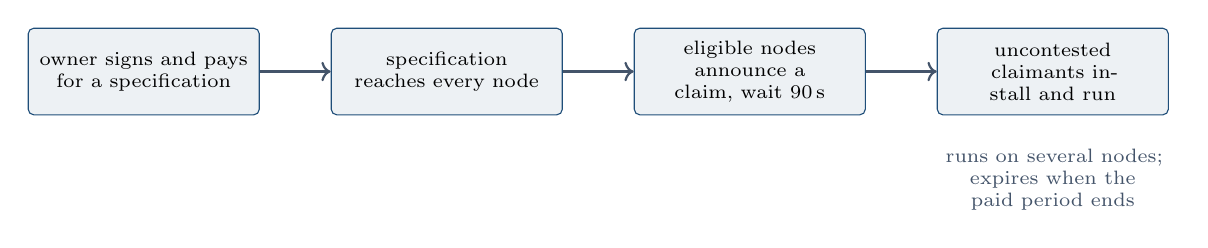
\begin{tikzpicture}[font=\small, node distance=9mm and 9mm,
  st/.style={draw=FluxBlue, fill=FluxBlue!8, rounded corners=2pt, minimum height=11mm,
             text width=27mm, align=center, font=\scriptsize},
  ar/.style={->, thick, FluxSlate}]
\node[st] (spec) {owner signs and pays for a specification};
\node[st, right=of spec] (bcast) {specification reaches every node};
\node[st, right=of bcast] (claim) {eligible nodes announce a claim, wait \SI{90}{\second}};
\node[st, right=of claim] (run) {uncontested claimants install and run};
\draw[ar] (spec) -- (bcast); \draw[ar] (bcast) -- (claim); \draw[ar] (claim) -- (run);
\node[below=3mm of run, font=\scriptsize, text=FluxSlate, text width=30mm, align=center]
  {runs on several nodes; expires when the paid period ends};
\end{tikzpicture}
\caption{From a signed specification to a running application. No account is opened at any step,
and no scheduler decides placement: nodes claim work, and a fixed wait resolves collisions.}
\label{fig:short:lifecycle}
\end{figure}

\subsection{Paying: a transaction, not a relationship}

Today, paying for a deployment means one thing: a single signed transaction, for the full price of
the period, to an address the chain knows. The price is a function of the resources reserved and the
duration --- CPU, memory, disk, instances, blocks --- and it is a \emph{reservation} price. You pay
for what you asked to hold, not for what you used. There is no metering, and therefore nothing to
meter, dispute, or attest.

When the paid period ends, the application stops. Renewing it is the owner's act, done the same way.
The protocol offers no subscriptions and no automatic renewal; operators who want that convenience
can buy it from a third-party service that holds a balance on their behalf, and the paper is
explicit that such a service is a business built on \Flux{}, not a feature of it.

\begin{figure}[H]
\centering
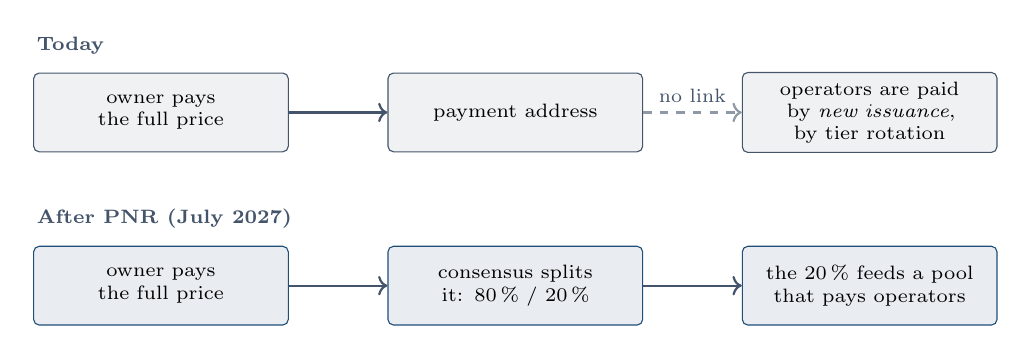
\begin{tikzpicture}[font=\small,
  box/.style={draw=FluxSlate, fill=FluxSlate!8, rounded corners=2pt, minimum height=10mm,
              text width=30mm, align=center, font=\scriptsize},
  hi/.style={box, draw=FluxBlue, fill=FluxBlue!10},
  ar/.style={->, thick, FluxSlate}, lbl/.style={font=\scriptsize, text=FluxSlate}]
\node[lbl, anchor=west] at (0,2.55) {\textbf{Today}};
\node[box] (t1) at (1.7,1.7) {owner pays the full price};
\node[box] (t2) at (6.2,1.7) {payment address};
\node[box] (t3) at (10.7,1.7) {operators are paid by \emph{new issuance}, by tier rotation};
\draw[ar] (t1) -- (t2);
\draw[ar, dashed, FluxSlate!60] (t2) -- node[above, lbl] {no link} (t3);

\node[lbl, anchor=west] at (0,0.35) {\textbf{After PNR (July 2027)}};
\node[hi] (p1) at (1.7,-0.5) {owner pays the full price};
\node[hi] (p2) at (6.2,-0.5) {consensus splits it: \SI{80}{\percent} / \SI{20}{\percent}};
\node[hi] (p3) at (10.7,-0.5) {the \SI{20}{\percent} feeds a pool that pays operators};
\draw[ar] (p1) -- (p2); \draw[ar] (p2) -- (p3);
\end{tikzpicture}
\caption{Where a payment goes. Today the money a tenant pays and the money an operator earns are
unconnected --- operators are paid by issuance. Under PNR, part of every payment flows into a pool
that pays operators instead. This is the hinge between the network as it is and as it is being
rebuilt.}
\label{fig:short:payment}
\end{figure}

\limitnote{The payment address is a single consensus-known address, and the split is applied by
consensus, not by the node software --- so a software release cannot change the distribution. What
the protocol does \emph{not} give a tenant is any remedy if a node fails to serve what was paid for.
Reservation pricing has no delivered-uptime quantity to compute a refund against, and the paper
records the decision that any such guarantee lives in the service layer, not the protocol.}

\section{What changes in v9}
\label{sec:short:changes}

Six changes, each with a date. Every one of them is planned rather than shipped unless the sentence
says otherwise, and the reader should hold that distinction throughout: this section describes a
network being rebuilt, and the full paper marks every element of it that is still undecided.

\subsection{Operators are paid by demand, not by issuance}

This is the change the others serve. Today an operator's income is new \flux{} minted every block;
the applications running on the network contribute nothing to it. Under \emph{Progressive Node
Rewards} that reverses: consensus takes \SI{20}{\percent} of every application payment on arrival
and pays it into a pool, and the pool drips into operator rewards over a rolling window of
\num{86400} blocks --- thirty days. The other \SI{80}{\percent} goes to the Foundation address that
already receives application payments today.

The split is applied by consensus at the address, not by any software a tenant or a node runs. The
pool balance is committed in every block and recomputed by every validator, so it cannot be
misreported. Activation is at block \textbf{\num{3787502}}, expected \textbf{1 July 2027}. That
height is not arbitrary: it is the block at which the parallel-asset mining allocation is exhausted,
computable today from the emission schedule, though no consensus constant encodes it yet; the
calendar date follows from the height at the thirty-second block target.

A reader should understand what this does and does not change. It changes \emph{where operator
income comes from} --- from issuance toward the workloads themselves. It does not, by design, pay a
node more for hosting more: every eligible node in a tier draws the same share of the pool
regardless of what it runs. The team chose that deliberately, because paying by placement would
turn the first-to-claim rule of \Cref{sec:short:how} into a race with money on it. The consequence
is stated in \Cref{sec:short:limits}.

\subsection{Ten parallel assets become two, on one redesigned bridge}

\Flux{} exists as a token on ten other chains. That footprint is being consolidated. Ethereum and
BNB Chain survive: balances there are carried across to new contracts by snapshot, and holders do
nothing. The other eight --- Base, Polygon, Avalanche, Ergo, Algorand, Solana, Tron and Kadena ---
are retired in stages: from March 2027 (block \num{3450000}) they become one-directional, with balances redeemable back to
the main chain and mining claims still collectable, but nothing swappable into them; the allocation
is cut in July, at the block where
it is exhausted and PNR activates; and in August (block \num{3880000}) the chains shut down, after which
unclaimed balances go to the Foundation. Ethereum and BNB Chain move to their new contracts earlier. What the height does
not settle is the balance already earned: roughly a quarter of what operators have accrued on these
chains has never been claimed, and the forfeiture rule is what closes that.

The numbers were measured rather than assumed, and they are reassuring in a way the raw supply
figures are not. Across all ten chains, \num{223027781.21}~\flux{} is actually held outside the
issuer's own addresses. Of that, \SI{97.21}{\percent} sits on the two surviving chains and needs
no holder action. Only \textbf{\num{6226900.80}~\flux{} --- \SI{2.79}{\percent}} --- is on the
retiring chains and exposed to the window.

The new bridge is mint-and-burn: minting on a parallel chain requires locked backing on the main
chain, so the total can never exceed what exists. It is guarded by a 3-of-4 signing quorum, a
1-of-4 emergency pause, a per-chain cap of \num{250000000}~\flux{}, a rate limit of
\num{10000000}~\flux{} per chain per day, and a 48-hour delay on any upgrade during which a
single guardian can cancel it. The quorum is held by four named people from one organisation,
and the paper says so.

\subsection{A new application specification}

Version 9 of the specification adds what the rest of this section needs: a duration expressed in
seconds rather than blocks, so lifetimes stop moving when block timing changes; a payment memo that
binds a payment to the application it funds, which is what lets PNR attribute revenue; and a
machine-type field that lets a specification ask for accelerated hardware. Enforcement is at block
\textbf{\num{3050000}}, expected in \textbf{late October 2026}, with existing applications migrated
automatically in the same quarter.

\limitnote{The fields are in the schema and not yet in the code that would act on them: as of the
survey, the payment memo, referral code and machine-type fields appear nowhere in the placement
path. The enforcement height is constrained to follow the implementation, not precede it.}

\subsection{The network can remove an application}

A collateral-weighted vote. Any node operator can file a report against an application on chain;
other operators vote by signing a transaction with their collateral key; if votes reach
\SI{25}{\percent} of the network's weight within a day, the next block carries a ban memo and every
node stops the application. The ban is final, the unused prepaid balance is burned, and the deployer
may return only as a new application. There is no appeal.

The team's stated position is that this is a network-level veto over content, not merely over
behaviour. That is a stronger power than any comparable network exercises, chosen knowingly, and its
principal risk is measured rather than hypothetical --- see \Cref{sec:short:limits}.

\subsection{Nodes that can prove what they are}

Two layers. The first is shipped: \ArcaneOS{}, the operating image nodes run, boots through a
measured chain --- Secure Boot, a pinned platform key, a hardware root, encrypted storage --- and
refuses to come up if any link fails. The second is planned: a bonded attestation network in which
nodes stake collateral on claims about what they serve, and lose it if a challenger proves them
wrong. Its parameters are set; its slashing construction, the paper is candid, is unsolved.

\subsection{The shielded pool is retired, and what that costs}

\Flux{}'s chain inherited Zcash's private-transaction machinery. It has been sealed to new entrants
since 2021 and today holds \num{96479.94}~\flux{} --- two hundredths of one percent of supply. The
decision is to retire it: announced now, sunset at block \num{3600000} in April 2027, before PNR
activates, and then remove the code. That makes the chain smaller, removes an inherited trusted
setup, and makes supply exactly auditable. It also means \textbf{\Flux{} will have no chain-level
privacy}: every payment will be publicly linkable, as on Bitcoin. The paper treats payment privacy
as an open problem from that point, not a delivered feature.

\subsection{And one change the fleet's own design forces}

A post-quantum note that is specific to \Flux{}. Because registering a node publishes the
collateral's public key on chain, \num{88514500}~\flux{} --- \SI{20.61}{\percent} of everything
issued --- sits in outputs a sufficiently capable quantum computer could spend immediately. Bitcoin's
comfort, that an unspent output hides its key, does not apply here. The adopted answer uses the one
lever \Flux{} has and Bitcoin does not: node collateral is a registered set that must keep
transacting to be paid, so migration to a post-quantum key can be made a condition of eligibility.
Operators who do not migrate stop earning; nothing is ever frozen.

\section{What it is for}
\label{sec:short:whatfor}

Everything so far has been description. This section is the argument: what a network of this shape
is good for, and why that is about to matter more than it did.

\subsection{The bet: the next tenant is software}

Open any cloud console today and you will find an interface built for a person. Pick a region. Choose
an instance size. Enter a card. Agree to terms. Every major cloud is built on the assumption that a
human is making the decision, and the whole surface --- accounts, billing relationships, credit
checks, support tiers --- follows from it.

\Flux{} is being rebuilt on the opposite assumption: that the caller is a program. Something that
provisions capacity when it needs it, pays for it, scales it, and releases it when the work is done,
with no human in the loop and no account anywhere.

The reason this is possible here and awkward everywhere else is narrow and concrete. On \Flux{},
paying for a deployment is a signed transaction. It is not a billing relationship. There is no
account to open, no card to hold, no legal entity to be. \textbf{A program can hold a key. It cannot
hold a corporate account.} That one asymmetry is the whole of the positioning claim, and everything
in this section follows from it.

This is not a prediction that people stop using clouds. It is a claim about where the growth goes.
Software that writes software, agents that run errands, pipelines that spin up a hundred short-lived
workers and vanish --- these are workloads whose natural interface is a key and a transaction, not a
console and an invoice.

\subsection{One substrate, and it already runs more than AI}

It would be easy, and wrong, to present \Flux{} as an AI network.

What actually runs on it today, by census rather than by aspiration, is a general-purpose mix:
ordinary web applications, blockchain infrastructure, content sites --- and \textbf{27 folding and
Rosetta deployments} doing real protein-folding and structural-biology work, which alone account for
roughly \SI{9}{\percent} of committed fleet CPU. Scientific simulation is not a use case \Flux{} is
hoping to attract. It is a use case that is already there, paying, at scale.

That matters more than it sounds, and the reason is economic rather than technical. A network that
serves only inference is idle whenever inference is idle. A network that serves web hosting,
scientific simulation, blockchain infrastructure and model inference --- from the same collateral,
the same placement, the same payment path --- has a demand base whose parts do not move together.
The generality is the resilience.

So the claim is not that \Flux{} becomes an AI cloud. It is that \Flux{} is a compute substrate on
which AI is one arriving workload class among several that are already running.

\subsection{Cloud and edge, converging}

\FluxCloud{} and \FluxEdge{} are to merge into a single product, offering accelerated compute through
one interface. A tenant should describe the work and let placement decide where it runs --- a
container on a commodity node, or a GPU on a datacenter machine --- without having to know which
product they are in. That convergence is planned, not shipped.

\limitnote{Convergence is at present an architectural intention with thin implementation behind it.
The only concrete artefact is a small, new capability specification, and the placement code that
would have to consume it does not read it yet: the three fields the new specification adds for this
purpose appear nowhere in the placement path. A merge announced is not a merge shipped, and this
document would rather say so than let a reader discover it later.}

\subsection{Why small models fit this fleet in particular}

The interesting question is not whether a decentralized network can run AI workloads. It is which
ones, and why.

Frontier-model inference is centralised for a specific engineering reason: the model does not fit on
one device, so it is sharded across many accelerators that must exchange activations at every layer.
That demands an interconnect --- machines physically close, wired together at bandwidths a wide-area
network cannot approach. A fleet of commodity machines scattered across the world is genuinely
unsuited to it, and no amount of decentralization enthusiasm changes that.

\textbf{But that requirement does not exist for a model that fits on a single device.} A model small
enough to sit in one machine's memory needs no interconnect at all, because there is nothing to
shard. The property that makes a dispersed fleet useless for frontier inference is simply absent for
the models most people actually need: the one that drafts the email, summarises the document,
triages the inbox, answers the question. Most work does not require a frontier model, and the work
that does not is precisely the work this shape of network can serve.

\begin{figure}[H]
\centering
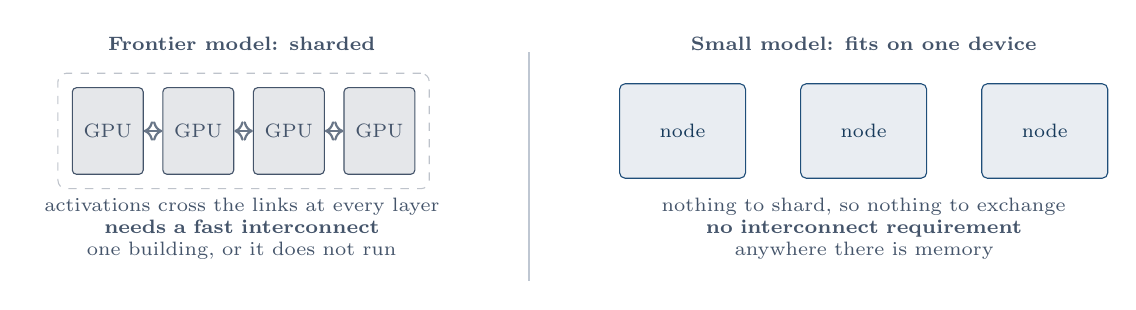
\begin{tikzpicture}[font=\small,
  gpu/.style={draw=FluxSlate, fill=FluxSlate!14, rounded corners=1.5pt,
              minimum width=9mm, minimum height=11mm, inner sep=1pt,
              font=\scriptsize, text=FluxSlate},
  fnode/.style={draw=FluxBlue, fill=FluxBlue!10, rounded corners=2pt,
                minimum width=16mm, minimum height=12mm, align=center,
                font=\scriptsize, text=FluxBlue!75!black},
  lbl/.style={font=\scriptsize, text=FluxSlate},
]
%% ---- left: sharded frontier inference ----
\node[lbl, anchor=south, font=\scriptsize\bfseries] at (2.7,2.05)
  {Frontier model: sharded};
\foreach \i/\x in {0/1.0,1/2.15,2/3.3,3/4.45} \node[gpu] (g\i) at (\x,1.15) {GPU};
\foreach \i/\j in {0/1,1/2,2/3} \draw[<->, thick, FluxSlate!80] (g\i) -- (g\j);
\begin{scope}[on background layer]
  \node[draw=FluxSlate!35, dashed, rounded corners=3pt, inner sep=5pt,
        fit=(g0)(g3)] (rack) {};
\end{scope}
\node[lbl, anchor=north, text width=52mm, align=center] at (2.7,0.42)
  {activations cross the links at every layer\\
   \textbf{needs a fast interconnect}\\
   one building, or it does not run};

%% ---- divider ----
\draw[FluxRule, thick] (6.35,-0.75) -- (6.35,2.15);

%% ---- right: single-device small model ----
\node[lbl, anchor=south, font=\scriptsize\bfseries] at (10.6,2.05)
  {Small model: fits on one device};
\node[fnode] (n0) at (8.3,1.15) {node};
\node[fnode] (n1) at (10.6,1.15) {node};
\node[fnode] (n2) at (12.9,1.15) {node};
\node[lbl, anchor=north, text width=58mm, align=center] at (10.6,0.42)
  {nothing to shard, so nothing to exchange\\
   \textbf{no interconnect requirement}\\
   anywhere there is memory};
\end{tikzpicture}
\caption{Why the constraint that centralises frontier inference does not bind here. Sharding a model
across accelerators forces them into one building; a model that fits on one device imposes no such
requirement, and a dispersed fleet stops being a disadvantage.}
\label{fig:short:interconnect}
\end{figure}

There is a second, sharper reason the fit is good, and it is a property of this fleet rather than of
decentralized networks generally. Decode speed follows a model's \emph{active} parameters, but
residency --- whether the model fits at all --- follows its \emph{total} parameters. Mixture-of-experts
models separate the two: they read only a few billion parameters per token while having to hold
tens of billions in memory. Such models therefore want \textbf{RAM} more than they want memory
bandwidth. RAM is what this fleet has, in quantity, across thousands of independent machines.

On commodity dual-channel hardware a four-billion-parameter quantised model runs at roughly
\num{12} tokens per second; on an eight-channel server, roughly \num{40}. Across the network's
tenant-available memory the capacity, at full utilisation, is on the order of tens of thousands of
concurrent small-model instances.

\limitnote{Those rates are a memory-bandwidth model --- achievable bandwidth divided by bytes read
per token --- and have \emph{not} been measured on \Flux{} hardware. A benchmark on each tier's
reference machines is scheduled for Q4~2026, and until it lands these are estimates rather than
results. The capacity figures are upper bounds at full utilisation, not availability: roughly
\SI{9}{\percent} of fleet CPU is already committed to the scientific workloads above. And the GPU
path has a harder limit --- accelerators are attached whole, with no subdivision, so a tenant wanting
a fraction of a card cannot have one, and a GPU request under contention is silently dropped rather
than refused.}

\subsection{What an autonomous tenant can and cannot do}

The agent story is the most likely place for a reader to assume more than is true, so it is worth
closing on precisely.

An agent on \Flux{} can hold a key, sign a deployment specification, pay for it, watch it run and
let it expire --- with no human, no account, and no intermediary at any step. That is real today for
the payment path, and it is the direct consequence of settlement being a transaction rather than a
relationship.

What an agent cannot be given is a spending limit the network enforces. \Flux{} inherits Bitcoin's
model, in which validating a transaction is a function of that transaction and the coins it spends
--- and nothing else. A rule like \emph{spend at most five \flux{} per day} requires knowing what the
key spent yesterday, and there is nowhere for that rule to live. \textbf{An agent's budget is
whatever you fund its key with, and that is the honest bound.} Anything richer needs a co-signer,
which puts back the intermediary the design exists to remove.

That is a real constraint and the paper states it rather than working around it. It is also, in
practice, a workable one: funding a key with what you are willing to lose is a familiar discipline,
and it fails closed.

\section{What we measured}
\label{sec:short:measured}

Every number in this document was retrieved from the network's own public interfaces on the dates
shown, and every one is reproducible by running the corresponding script in the public repository.
This is the credibility of the document, so it is stated compactly and without interpretation.

\begin{center}\small
\begin{tabular}{@{}lrl@{}}
\toprule
Quantity & Value & Retrieved \\
\midrule
Nodes, all tiers & \num{6489} & 2026-09-03 \\
\quad Cumulus / Nimbus / Stratus & \num{3247} / \num{1615} / \num{1627} & 2026-09-03 \\
Collateral locked & \num{88514500}~\flux & 2026-09-03 \\
Applications deployed & \num{1195} & 2026-09-03 \\
\quad on specification v8 & \num{873} (\SI{73.05}{\percent}) & 2026-09-03 \\
\quad scientific-simulation deployments & \num{27} & 2026-09-03 \\
Issued main-chain supply & \num{429466823.97}~\flux & height \num{2912015} \\
Shielded pools, Sprout $+$ Sapling & \num{96479.94}~\flux & height \num{2917115} \\
Parallel-asset liability, all ten chains & \num{223027781.21}~\flux & 2026-09-03/04 \\
\quad exposed to the redemption window & \num{6226900.80}~\flux{} (\SI{2.79}{\percent}) & 2026-09-03/04 \\
Proof of Node activation & block \num{2020000} & 2025-10-25 \\
\bottomrule
\end{tabular}
\end{center}

Two of these were harder to obtain than they look, and are worth a sentence each because they
correct impressions the raw figures give.

\textbf{Parallel-asset liability is not total supply.} Each parallel asset was minted at its full
nominal amount --- \num{440000000} on most chains --- and the issuer still holds nearly all of it.
The figure that matters for consolidation is what left the issuer's hands, which required the
issuer's own address registry to compute. On Solana, for instance, nominal supply is sixty million
and the outstanding balance is \num{373067.20}.

\textbf{Two chains needed a different method.} Kadena's token contract exposes no total-supply
function; supply was recovered by enumerating every account across its twenty chains and summing.
Tron required the block explorer's API rather than the node's. Both are scripted.

\limitnote{The table states what is public. It does not state utilisation, which no public interface
reports; per-owner concentration beyond what the chain exposes, which needs beneficial-ownership
data; or real token rates for inference, which are scheduled to be measured in Q4~2026. Where a
number is absent here, it is because it could not be established rather than because it was not
looked for.}

%% Starts a fresh page: the table below is too tall to share one with a stranded heading.
\clearpage
\section{What does not work yet}
\label{sec:short:limits}

A document that only said the first five sections would be a pitch. This one is the reason to
believe the rest. Each row is a finding from the full paper, stated once and without softening; the
last column is what, if anything, is being done about it.

\begin{center}\small
\renewcommand{\arraystretch}{1.25}
\begin{tabular}{@{}>{\raggedright\arraybackslash}p{3.15cm}p{4.85cm}p{5.2cm}@{}}
\toprule
& The limit & Why it matters, and the response \\
\midrule
\textbf{Hosting pays nothing extra} &
PNR pays every eligible node in a tier the same share, regardless of what it runs. The marginal
reward for hosting an application is exactly zero. &
Free-riding is individually rational; what compels hosting is the eligibility gate, and that gate is
currently bound to neither the operator nor the machine. This is deliberate --- paying by placement
would make the claim race a race for money --- and the answer is attested execution, which is why
that work is a precondition rather than a follow-on. \\
\textbf{Four parties reach the removal threshold} &
At the measured collateral distribution, four owner identities together hold \SI{25}{\percent} of
voting weight. The moderation quorum is not censorship-resistant today. &
Accepted knowingly, with growth as the expected remedy. The paper notes the tension: the network's
answer to weak demand is contraction, and contraction concentrates. Censorship resistance is, in
effect, a function of demand for the cloud. \\
\textbf{No chain-level privacy} &
The shielded pool is being retired. Every payment will be publicly linkable. &
A deliberate trade for a smaller, auditable chain. Payment privacy becomes an open problem, and the
paper says so rather than claiming otherwise. \\
\textbf{One discovery endpoint} &
The service that tells the network which applications exist and where they run is a single
Foundation-operated API, with no on-chain or peer-to-peer fallback. &
If it goes down, nothing new propagates; the last-known configuration keeps serving. A real
control-plane single point of failure, stated in the full paper's centralisation inventory. \\
\textbf{Four keys can produce blocks} &
An emergency path lets a 2-of-4 key set produce blocks that bypass the node-eligibility check, with
no time or stall-detection gating on when it may be used. &
Intended for recovery from a stalled chain, and the set is planned to move to 3-of-4 with fresh
keys. But the gating is absent at either size: nothing in consensus limits \emph{when} the path
fires, only \emph{who} can fire it. The full paper lists it in the centralisation inventory
alongside the discovery endpoint. \\
\textbf{The bridge is administered} &
Mint, release and upgrades are 3-of-4 among four people from one organisation, and the contracts
are upgradable. &
Explicitly a bring-up safety net, with immutability the stated destination once a third-party audit
and a proven operating record exist. Until the upgrade path is renounced on chain, the paper
describes the bridge as administered, not trust-minimized. \\
\textbf{Accelerators attach whole} &
A GPU is passed through as an entire device. There is no subdivision, and a request under
contention is silently dropped rather than refused. &
This is the one thing the small-model thesis of \Cref{sec:short:whatfor} needs and the current
allocation cannot do. Planned with the cloud/edge merge; not shipped. \\
\bottomrule
\end{tabular}
\end{center}

None of these is hidden in the full paper, and none should be hidden here. A reader deciding whether
to run a node, deploy an application, or build on this platform is better served by knowing them
than by discovering them.

\section{Where this goes}
\label{sec:short:where}

\subsection{The dates}

\begin{figure}[H]
\centering
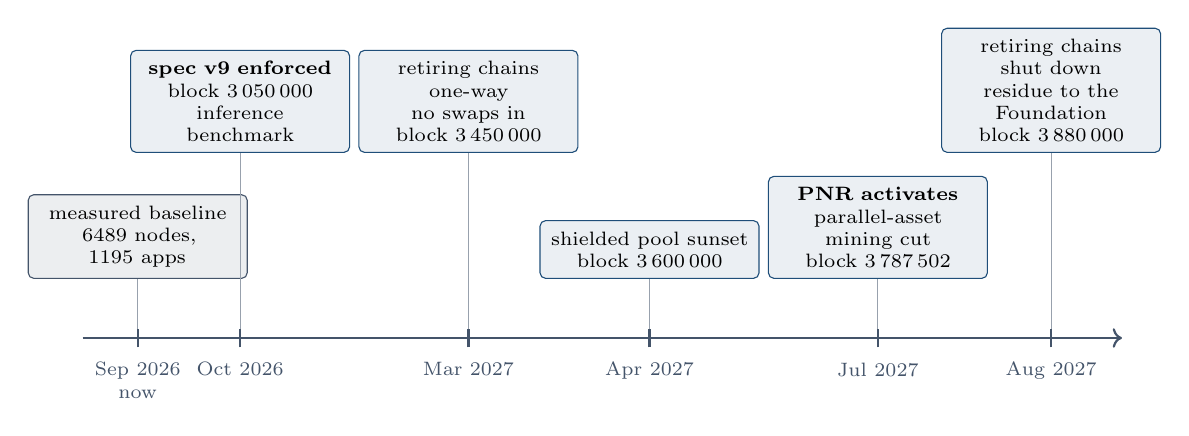
\begin{tikzpicture}[font=\scriptsize,
  ev/.style={draw=FluxBlue, fill=FluxBlue!9, rounded corners=2pt, text width=25mm,
             align=center, inner sep=4pt},
  now/.style={draw=FluxSlate, fill=FluxSlate!10, rounded corners=2pt, text width=25mm,
              align=center, inner sep=4pt},
  tick/.style={FluxSlate, thick}, lead/.style={FluxSlate!55, thin}]
%% Axis fits the text block; events alternate between two heights so that
%% neighbouring boxes cannot collide however long their labels run.
\draw[->, thick, FluxSlate] (0,0) -- (13.2,0);
\foreach \x/\l in {0.7/{Sep 2026\\now}, 2.0/{Oct 2026}, 4.9/{Mar 2027}, 7.2/{Apr 2027}, 10.1/{Jul 2027}, 12.3/{Aug 2027}}
  {\draw[tick] (\x,-0.12) -- (\x,0.12);
   \node[below=2pt, text=FluxSlate, align=center] at (\x,-0.12) {\l};}
%% low row
\draw[lead] (0.7,0.12) -- (0.7,0.75);
\node[now, anchor=south] at (0.7,0.75) {measured baseline\\ \num{6489} nodes, \num{1195} apps};
\draw[lead] (7.2,0.12) -- (7.2,0.75);
\node[ev,  anchor=south] at (7.2,0.75) {shielded pool sunset\\ block \num{3600000}};
\draw[lead] (10.1,0.12) -- (10.1,0.75);
\node[ev,  anchor=south] at (10.1,0.75) {\textbf{PNR activates}\\ parallel-asset\\ mining cut\\ block \num{3787502}};
%% high row
\draw[lead] (2.0,0.12) -- (2.0,2.35);
\node[ev,  anchor=south] at (2.0,2.35) {\textbf{spec v9 enforced}\\ block \num{3050000}\\ inference benchmark};
\draw[lead] (4.9,0.12) -- (4.9,2.35);
\node[ev,  anchor=south] at (4.9,2.35) {retiring chains one-way\\ no swaps in\\ block \num{3450000}};
\draw[lead] (12.3,0.12) -- (12.3,2.35);
\node[ev,  anchor=south] at (12.3,2.35) {retiring chains shut down\\ residue to the Foundation\\ block \num{3880000}};
\end{tikzpicture}
\caption{The dated schedule. Heights are consensus facts and calendar dates assume the thirty-second
block target holds. Everything to the right of ``now'' is planned.}
\label{fig:short:timeline}
\end{figure}

Three things are true about this schedule and worth stating together. The heights are fixed and
public, so anyone can check whether they were met. The order is deliberate: the specification
change lands roughly eight months before the economic change that depends on it, so the fields PNR
needs have time to prove themselves. And the whole sequence is falsifiable --- the full paper names,
for each milestone, the public observation that would show it had not happened.

\subsection{How to participate}

\textbf{Run a node.} Lock the collateral for a tier, run the node software on hardware that clears
that tier's benchmark, and the chain does the rest. Income today is issuance by rotation; from July 2027 it is issuance plus a share of application revenue. What you cannot do is earn more by hosting
more --- see \Cref{sec:short:limits} before deciding that is what you want.

\textbf{Deploy an application.} Write a specification, sign it, pay for it. There is no account and
no approval step. The application runs on several nodes until the paid period ends, and renewing it
is your act. If you want subscriptions and cards, a third-party service offers them on top; the
protocol does not.

\textbf{Build for machines.} If your tenant is a program --- an agent, a pipeline, a system that
provisions and releases capacity on its own --- \Flux{} is being built for exactly that caller. Give
it a key, fund the key with what you are willing to lose, and it needs nothing else from anyone.

\textbf{Read the source.} The chain, the node software and the tooling are public repositories, and
the full paper cites them by file and line for every claim about behaviour. Where it cites a private
repository, it says so.

\section*{Read further}
\addcontentsline{toc}{section}{Read further}
\markboth{Read further}{}
\label{sec:short:further}

This document is a door into a longer one. \emph{Flux v9: A Decentralized Cloud for Autonomous
Compute} runs to over four hundred pages, cites source code by file and line for every claim about
deployed behaviour, proves what can be proved, and marks every undecided element as such. Nothing
here goes beyond it; everything here is compressed from it. If a claim in this document seems too
strong, too weak, or too neat, the section below is where to check.

\begin{center}\small
\begin{tabular}{@{}p{5.2cm}p{8.4cm}@{}}
\toprule
If you want\ldots & \ldots read, in the full paper \\
\midrule
the system model and the adversary it is defended against & \S2, System model \\
the network as measured, with methodology & \S3, Flux as deployed today; \S25, Evaluation \\
how Proof of Node works, and why fork choice is a block-count race & \S4, Consensus \\
the full emission schedule and supply function & \S5, Monetary policy; Appendix C \\
the parallel-asset measurement, chain by chain & \S6, Parallel assets \\
PNR specified: the pool, the drip, the invariants, and why hosting pays nothing extra & \S7, Progressive Node Rewards \\
how placement actually works, with the ninety-second rule & \S9, FluxOS \\
the v9 specification and what consumes it & \S10--\S11 \\
the boot chain, and what a tenant can and cannot verify & \S14, Attested execution \\
the small-model argument, with the capacity estimates and their caveats & \S15, Accelerated compute \\
what an agent can hold, sign and be bounded by & \S17--\S18 \\
the bridge construction, its invariants, and the quorum's limits & \S22, Trust-minimized bridging \\
the moderation quorum and the concentration measurement & \S23, Governance \\
the shielded pool, its retirement, and the post-quantum finding & \S20, \S8 \\
everything that does not hold, in one place & \S28, Limitations \\
\bottomrule
\end{tabular}
\end{center}

The full paper, its evidence corpus, and every script that produced a number in either document are
in the public repository.


\end{document}
